% !TEX TS-program = pdflatex
% !TEX encoding = UTF-8 Unicode

% This is a simple template for a LaTeX document using the "article" class.
% See "book", "report", "letter" for other types of document.

\documentclass[12pt,final,oneside]{memoir} % use larger type; default would be 10pt

\usepackage[utf8]{inputenc} % set input encoding (not needed with XeLaTeX)
\usepackage[margin=2cm]{geometry}
\usepackage{xy}
\usepackage{amsmath, amsthm}
\usepackage{showkeys}
\usepackage[smaller]{acronym}
\usepackage[marginclue]{fixme}
%\usepackage{natbib}
\usepackage{tabularx}
\usepackage{chngpage}
\usepackage{booktabs}
\usepackage{cite}
\usepackage{times}
\usepackage{graphicx}
\usepackage{ctable}
\usepackage{footnote}
\usepackage{amssymb}
\usepackage{url}
\usepackage{tikz-timing}
\usepackage[lofdepth,lotdepth]{subfig}
\usepackage{multirow}
\fxsetup{
    status=final,
    author=,
    layout=marginclue,inline, % also try footnote or pdfnote
    theme=color
}
\definecolor{fxnote}{rgb}{0.8000,0.0000,0.0000}

\OnehalfSpacing
\setcounter{tocdepth}{3}

\usepackage{color}
\usepackage{listings}
\lstset{ %
language=C++,                % choose the language of the code
basicstyle=\ttfamily,       % the size of the fonts that are used for the code
numbers=left,                   % where to put the line-numbers
numberstyle=\footnotesize,      % the size of the fonts that are used for the line-numbers
stepnumber=1,                   % the step between two line-numbers. If it is 1 each line will be numbered
numbersep=5pt,                  % how far the line-numbers are from the code
backgroundcolor=\color{white},  % choose the background color. You must add \usepackage{color}
showspaces=false,               % show spaces adding particular underscores
showstringspaces=false,         % underline spaces within strings
showtabs=false,                 % show tabs within strings adding particular underscores
frame=single,           % adds a frame around the code
tabsize=2,          % sets default tabsize to 2 spaces
captionpos=b,           % sets the caption-position to bottom
breaklines=false,        % sets automatic line breaking
breakatwhitespace=false,    % sets if automatic breaks should only happen at whitespace
escapeinside={\%*}{*)}          % if you want to add a comment within your code
}

%%% END Article customizations

%%% The "real" document content comes below...

\title{VPR Assessment of a Novel Partitioning Algorithm}
\author{David Munro}
%\date{} % Activate to display a given date or no date (if empty),
         % otherwise the current date is printed

\begin{document}
\maketitle
\begin{abstract}
	\ac{FPGA} systems would be well suited to space based applications except for their vulnerability to space based radiation. Various techniques for dealing with their susceptibility have been discussed in literature. This thesis aims to implement and assess a key part of a theoretical technique to protect against radiation induced \acp{SEU} and assess the overheads of said technique.
\acresetall
\end{abstract}
\chapter*{Acknowledgements}
Thanks go to...

\tableofcontents*
\newpage

\begin{acronym}[printonlyused,withpage]
\acro{VPR}[VPR]{Versatile Place and Route}
\acro{MCNC}[MCNC]{Microelectronics Centre of North Carolina}
\acro{BLE}[BLE]{Basic Logic Element}
\acro{CLB}[CLB]{Configurable Logic Block}
\acro{DFG}[DFG]{Directed Flow Graph\acextra{or a DataFlow Graph}}
\acro{SEU}[SEU]{Single Event Upset}
\acro{LUT}[LUT]{Look Up Table}
\acro{VTR}[VTR]{Verilog To Routing}
\acro{STL}[STL]{Standard Template Library}
\acro{FPGA}[FPGA]{Field Programmable Gate Array}
\acro{TMR}[TMR]{Triple Modular Redundancy}
\acro{BLIF}[BLIF]{Berkeley Logic Interchange Format}
\acro{ASIC}[ASIC]{Application Specific Integrated Circuit}
\acro{LAB}[LAB]{Logic Array Block}
\acro{IO}[I/O]{Input/Output}
\acro{ICAP}[ICAP]{Internal Configuration Access Port}
\acro{SRAM}[SRAM]{Static RAM}
\acro{mux}[mux]{Multiplexer}
\acro{CAD}[CAD]{Computer Aided Design}
\acro{MBU}[MBU]{Multi Bit Upset}
\acro{NRE}[NRE]{Non Recurring Engineering}
\acrodef{DICE}[DICE]{Dual Interlock Storage Cell}
\acrodef{SIS}[SIS]{SIS}
\acused{SIS}
%\acrodef{EEPROM}[EEPROM]{EEPROM}
\end{acronym}
\chapter{Introduction}
\section{Overview}
Space plays an increasingly important role in the functioning of modern societies, being vital for fields including navigation, meteorology, and communications\cite{OECDSpace}. \acl{FPGA} systems (\acsp{FPGA}) have many beneficial features, such as their flexibility and low \ac{NRE} costs which make them highly desirable for space based applications except for their greater susceptibility to space radiation. Hardened \acp{FPGA} offer only a fraction of the gate counts (and hence capability of implementing large or complex circuits) of non hardened offerings prompting a search for a solution to the radiation susceptibility of \acp{FPGA} using mainstream hardware\cite{VFPGATMR}, one of the most popular of which is \ac{TMR}. In \ac{TMR}, vulnerable components are triplicated allowing for errors to be detected and mitigated. This thesis is based on the work of\cite{DiesselChange} which introduces an approach to \ac{TMR}, and aims to implement a key part of the approach and assess the implementation with the aid of an open source \ac{CAD} toolchain for \acp{FPGA}.
The remainder of this chapter provides an overview of these technologies, discusses alternatives to our approach, and details why we have chosen the technique we have. Chapter 2 introduces our approach to benchmarking circuits, and presents our initial results along with a brief discussion; Chapter 3 describes our implementation and design choices made in the implementation and Chapter 4 outlines our schedule and current progress, and our final chapter presents our closing remarks.
\acresetall
\subsection{\acsp{FPGA}}
\acp{FPGA} are popular devices capable of implementing a wide variety of circuits. Unlike \acp{ASIC} which must be specially designed and manufactured for an application---a lengthy and expensive process---\acp{FPGA} are a generic off the shelf device which can be mass produced by manufacturers and then adapted for an individual user's needs. Their flexibility, low cost, and faster development time make them the most economic for a number of applications.


\fxnote{TODO: Use own image. Wilton lecture notes have no license/copyright notice/etc attached, so don't know if this usage is actually allowed. Plus, doesn't look that good.}
\begin{figure}
    \begin{center}
        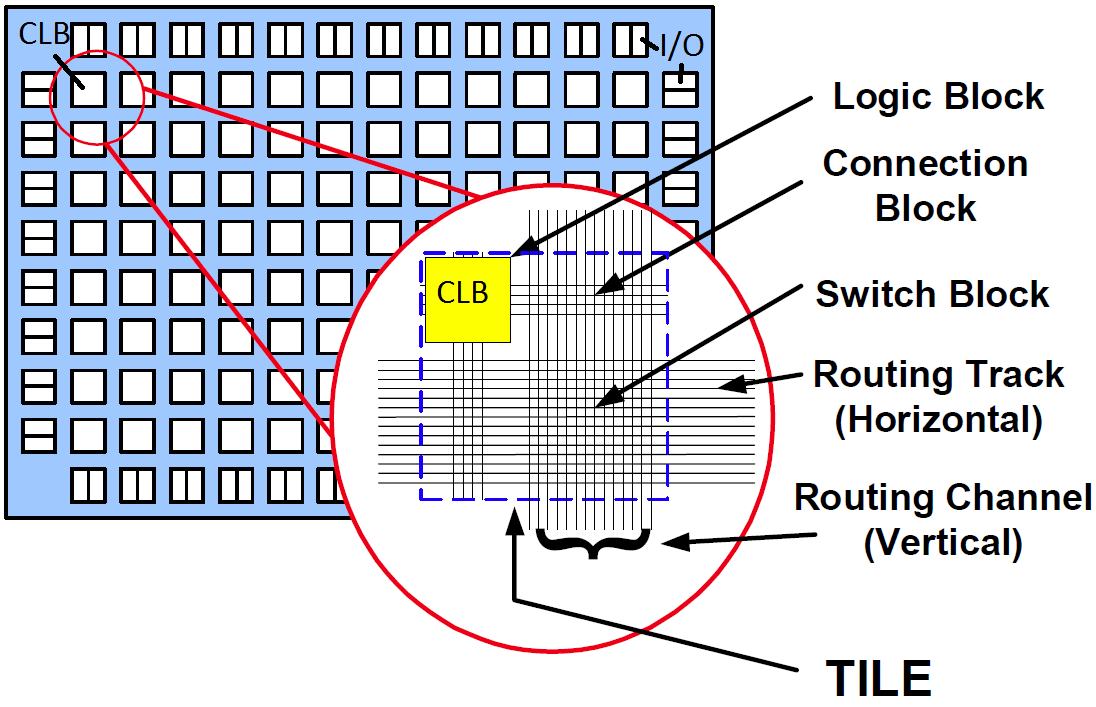
\includegraphics[width=0.6\textwidth]{images/fpga-arch.png}
        \caption{Island Style FPGA\cite{WiltonLecture}}
        \label{FPGAArch}
    \end{center}
\end{figure}

There are three main components to an \ac{FPGA}: \ac{IO} blocks, usually around the edge, allowing for input and output from the \ac{FPGA}, \acp{CLB} containing all the logic elements or \emph{primitives}, and the routing between everything.
Most \acp{FPGA} also contain other structures embedded in the \ac{CLB} array to provide commonly used resources such as multipliers. While they can be implemented using latches and \acp{LUT}, embedding them as discrete components allows for denser designs.
The routing between componenets consists of channels running horizontally and vertically with a number of wires and programmable switches connecting the wires to each other and to \acp{CLB} allowing for configurable paths between arbitrary components. A typical switch or connection block has a configuration cell storing the state, and a connection can be made or unmade by writing a new value to the cell for that switch. The most common style of routing is known as island style (as the \acp{CLB} are located as islands in a sea of routing) with the routing area making up some 80\%-90\% of the \ac{FPGA}'s area\cite{FPGAArch}.
Each \ac{CLB} is a cluster of smaller blocks, called \acp{BLE}, with each \ac{BLE} containing the logic primitives, typically a programmable \ac{LUT} to implement combinational logic, a latch for register operations and implementing sequential logic, and a \ac{mux} to switch between the two. As with the switches in routing the values for the \ac{LUT}, whether the \ac{mux} is selecting the latch or \ac{LUT} output, and other component states are all stored in configuration memory, typically implemented in \acs{SRAM}.

Programming an \ac{FPGA} involves loading in a bitstream which describes all the component values (i.e. contents of the configuration memory for each cell) for a circuit, accomplished through writing the bitstream to a special configuration port on the \ac{FPGA}. A number of \acp{FPGA} also allow for run time programming, or reconfiguration, of parts of a circuit through loading the bitstream for only the section of interest while the rest of the \ac{FPGA} keeps running.

\fxnote{Check grammar in this next section.}
There are four main technologies used to implement the configuration memory in \acp{FPGA}:
\begin{itemize}
\item \ac{SRAM}, which gives the highest density devices and includes the Virtex-5 family this thesis focuses on; however they are volatile and must be reprogrammed every power up from an external configuration memory;
\item (anti)fuse, which are only one time programmable;
\item flash, which is non-volatile (thus not requiring an external configuration memory) and reprogrammable; however has a lower density than \ac{SRAM} based \acp{FPGA}\cite{FPGAArch}.
\end{itemize}
\subsubsection{Partial Reconfiguration}
Partial reconfiguration involves loading configuration information for part of a circuit during operation. Much like the complete configuration described above, it involves writing a configuration bitstream to one of the available configuration ports, in this case also including the location to reconfigure. The configuration memory of recent Virtex devices is split into frames, and one can only reconfigure entire frames. A configuration frame is 41 (32-bit) words long on a Virtex-5 device and configures a bit slice of the device that spans 20 \ac{CLB} rows. As more frames are being reconfigured the larger the bitstream, and consequently the longer the time to reconfigure. The main configuration ports used are the external SelectMAP interface, or the internal \ac{ICAP}, each with a bandwidth of 400MB/s in all Virtex devices \cite{XCell33,DiesselChange}


\subsection{Space Based Applications}
Space is quite different from a terrestrial environment, and \acp{FPGA} have a number of advantages due to their lower \ac{NRE} costs and flexibility. As \acp{FPGA} can be reconfigured during a mission, faulty or outdated designs can be replaced remotely; however, there is a significant downside: as systems go further into space and are no longer protected by the earth's atmosphere they become increasingly likely to suffer from radiation induced errors where ionising radiation intersecting with a component causes charge build up, potentially triggering incorrect operation\cite{SEEMechanism}. As outlined in Table \ref{SEURate}, for higher orbits the mean time to upset is on the order of only a second, and this rate increases as technology advances and chip density further increases.
\begin{table}
    \begin{center}
        \begin{tabular}{lll}
        \toprule
        Orbit & SEUs per device/day &Mean time to upset (s)\\
        \midrule
        LEO (560 km) & 4.09 & 2.11 $\times 10^4$\\
        Polar (833 km) & 1.49 $\times 10^4$ & 5.81\\
        GPS (20,200 km) & 5.46 $\times 10^4$ & 1.58\\
        Geosynchronous (36,000 km) & 6.20 $\times 10^4$ & 1.39\\
        \bottomrule
        \end{tabular}
        \caption{SEU Rate Predictions for Virtex-4 devices at various orbits\cite{DiesselChange}}
        \label{SEURate}
    \end{center}
\end{table}
Of the potential effects, which range from unnoticeable to device destruction, this thesis is concerned with mitigating \acp{SEU}, where an incorrect signal is triggered but the underlying circuitry is not damaged. We also concern ourselves primarily with errors affecting only single bits or components rather than \acp{MBU} in which multiple components are affected at the same time.

%\begin{table}
%    \subfloat[][ASIC]{
%        \begin{tikztimingtable}
%        Expected Output & LLLLLLLLL\\
%        Actual Output   & LLLLLHLLL\\
%        \end{tikztimingtable}
%    }
%
%    \subfloat[][FPGA]{
%        \begin{tikztimingtable}
%        Expected Output & LLLLLLLLL\\
%        Actual Output   & HHHHHHLLL\\
%        \end{tikztimingtable}
%    }
%    \label{ASICVFPGA}
%\end{table}
In an \ac{ASIC}, while \acp{SEU} may be picked up and latched, or otherwise continue affecting the circuit in future, the component itself continues operating normally.

\acp{FPGA} on the other hand are vulnerable to configuration errors as well. When the charged particle impacts configuration memory it can flip the state of that cell changing the actual circuit. Unlike transient errors, these functional errors persist until corrected.

Additionally for \ac{SRAM} devices, the off-chip configuration memory itself can be affected, so the next time the chip is reprogrammed (e.g. after power cycling), an incorrect circuit configuration will be loaded.

(Anti)fuse devices, being non reprogrammable, are immune to configuration errors, though both \ac{SRAM} and flash based \acp{FPGA} are vulnerable and all three are susceptible to transient \ac{SEU}\cite{HFPP}.

\subsection{How We Deal With \acs{FPGA} Downsides}
Clearly, in order for \acp{FPGA} to be viable in space based systems the effects of \acp{SEU} must be mitigated. A number of technologies and techniques are available, each with their own advantages and disadvantages. A number of options exist which detect errors but are unable to determine the correct result, requiring a reload of the configuration memory while the circuit is non operational until the reconfiguration completes. For many applications this downtime is impractical, thus we will be looking at options which allow the circuit to continue operating correctly.
There are three main categories of \ac{SEU} hardening techniques\cite{HardeningTechniques}:
\begin{itemize}
    \item Charge Dissipation, which aims to keep the effect of the radiation below the level where it would have an effect. This includes techniques such as increasing the drive current. These methods typically require custom hardware (increasing costs) and usually increase power usage.
    \item Temporal Filtering, which aims to filter out transient \acp{SEU}, includes methods such as delay-and-vote\cite{HardeningTechniques}. These techniques often slow down operation and are ineffective against configuration errors.
    \item Spatial Redundancy, which uses multiple redundant circuits to detect errors and be able to continue operating. Spatial redundancy techniques include \ac{DICE}\cite{DICE} and \ac{TMR} and can be implemented either in hardware or at the design level not requiring any custom hardware. These methods typically increase area and power usage.
\end{itemize}
While hardened \acp{FPGA} are available, they typically lag well behind mainstream commercial offerings\cite{VFPGATMR}, thus solutions which can be implemented on mainstream commercial \ac{FPGA} hardware are desirable. Additionally, there is very little point hardening an \ac{FPGA} and not its configuration buffers and memory which take up far more surface area\cite{FPGAArch} and are thus even more vulnerable.
For these reasons \ac{TMR}, requiring no custom hardware and providing \ac{SEU} protection against both transient and functional errors, is one of the more popular \ac{SEU} hardening techniques even though it comes at the cost of more than tripling area and greatly increasing power usage.

\begin{table}
    \begin{tabularx}{\textwidth}{X|XXXl}
    \toprule
   & POWER & SPEED & HARDNESS (e/b-d) & AREA ($\mbox{mm}^2$)\\
   \midrule
Std Low Power & Rise – 0.7 $\mu$ W \newline Fall – 0.2 $\mu$ W & Rise – 0.21 ns \newline Fall – 0.27 ns & $10E-8$ \newline 1 node & 360\\
   \midrule
Increased IDRIVE & Rise – 1.0 $\mu$ W \newline Fall – 0.2 $\mu$ W & Rise – 0.16 ns \newline Fall – 0.15 ns & $2\times10E-9$ \newline 1 node & 460\\
   \midrule
\ac{TMR} & Rise – 1.72 $\mu$ W \newline Fall – 1.27 $\mu$ W & Rise – 0.21 ns \newline Fall – 0.27 ns & $10E-11$ \newline 2 node & 1200\\
   \midrule
DICE & Rise - 1.4$\mu$ W \newline Fall - 1.1$\mu$  W & Rise - 0.96 ns \newline Fall - 0.97ns & $1.6\times10E-10$ \newline 2 node & 520 \\
\bottomrule
\end{tabularx}
    \caption{Comparison of hardening techniques\cite{HardeningTechniques}\fixme{Explain columns}}
    \label{HardeningComparison}
\end{table}

One additional technique specific to \ac{SRAM} based \acp{FPGA} relates to the protection of the off-chip configuration memory. As \ac{SRAM} is volatile and loads the state from off chip at power up, this external configuration memory must also be protected from \acp{SEU}. This can be accomplished by incorporating error detection and correction techniques in the RAM, something already in place on a number of mainstream \acp{FPGA} such as the Virtex-4 and -5\cite{DuttonSEU}.


\section{\acl{TMR}}
\fixme{Explain better, see Diessel comments}
Triple Modular Redundancy is a commonly used method for creating fault tolerant systems in which a given circuit is implemented three times with independent components, with the outputs feeding into a voter circuit to determine the majority value. Any \ac{SEU} will affect the output value of at most one version, so the majority vote is still correct. For transient errors that are not in a feedback loop correcting the output is enough to fix the error; however \acp{SEU} in feedback paths or in the configuration memory will persist, and this require some method for eliminating them. One possible approach is resetting the system, however while this occurs the system is unavailable so a reset may not be a feasible solution. Instead, partial reconfiguration can reconfigure only the faulty circuit while the redundant circuits continue operating and providing output. After reconfiguration the circuit must then be resynchronised to the same state as the other two. We use the approach presented by \cite{DiesselChange} which involves running the circuit until the state converges, which is guaranteed to occur within a timeframe given by the number of register stages and the clock frequency. In order for this approach to guarantee resynchronisation the circuit must be acyclic: there can be no feedback loops which may carry incorrect data. To solve this we simply ensure that all feedback loops are \emph{cut}, that is, the value is voted on before being passed back into the circuit. This has the additional benefit of correcting transient errors which would otherwise be caught in a feedback cycle, by ensuring the cycle data is correct.
 
 
 
 
 
 
 This on its own is enough for transient errors, assuming they and one can then incorporate partial reconfiguration in order to recover from detected errors; however, this only works when at most one \ac{SEU} occurs within the error detection and recovery time; Should \acp{SEU} occur in two of the three partitions then it is impossible for the voter to determine the correct value, necessitating a complete reload of the configuration memory (\emph{scrubbing}). Therefore, we require the error detection and recovery time to be sufficiently small that the likelihood of multiple events occurring within that time period are negligible.
Once the error has been detected and the circuit reconfigured it must then be resynchronised with the other partitions. For this thesis we will assume a method similar to that described in\cite{DiesselChange}, where the resynchronising circuit is run on the same input for a number of steps equal to the number of register stages so no potentially incorrect data is left in the pipeline, but our implementation will work for any method where Equation \ref{ERT} holds.
The error recovery time consists of the time to reconfigure the circuit, which is a function of the circuit area, and the resynchronisation time, which is a function of the number of register stages and clock frequency, so it is required that our area and number of register stages are small enough, and frequency large enough, that our error recovery time is within a user specified limit.
\begin{align}
    \mbox{Error Recovery Time} &=\mbox{Error Detection Time} + \mbox{Reconfiguration Time} + \mbox{Resynchronisation Time}\notag\\
    \mbox{Error Detection Time} &<= \frac{1}{\mbox{Clock Frequency}}\times\mbox{Register Stages}\notag\\
    \mbox{Reconfiguration Time} &= \frac{1}{\mbox{Reconfiguration Speed}}\times\mbox{Bitstream Size}+Constant\notag\\
     &\propto \mbox{Partition Size in Frames}\notag\\
    \mbox{Resynchronisation Time} &<= \frac{1}{\mbox{Clock Frequency}}\times\mbox{Register Stages}\notag\\
    \therefore \mbox{Error Recovery Time} &<= \frac{2\times\mbox{Register Stages}}{\mbox{Clock Frequency}} + \frac{\mbox{Bitstream Size}}{\mbox{Reconfiguration Speed}}+Constant\label{ERT}
\end{align}\cite{DiesselChange}
Additionally, as each voter circuit adds some constant overhead in terms of area, power usage and clock frequency slowdown it is desirable to have each partition as large as possible. This thesis is concerned with implementing and assessing this \ac{TMR} design; a discussion of other \ac{TMR} methods and our reasons for not using them is included below.
\subsection{\acl{TMR} Implementations}
This thesis builds on the work of\cite{DiesselChange} which details a partitioning algorithm that traverses a circuit represented as a \ac{DFG} in a breadth first manner, creating partitions that stay within our constraints.
Our goal is to create an algorithm which stays within a user specified error recovery time, doesn't require existing code to be rewritten, allows for both custom voting and reconfiguration logic to be added, can use industry standard \acp{FPGA} rather than custom hardware, and effectively protects the entire system from \acp{SEU} with as close to no downtime as achievable. There are a number of existing \ac{TMR} solutions, however none quite meet our requirements.
Our first requirement is that standard \ac{FPGA} hardware can be used, with our implementation specifically targeting Virtex 5 chips. Options with custom hardware such as \cite{VFPGATMR} (with three \acp{FPGA} and an \ac{ASIC} voter in a single package), are often prohibitively expensive, and prevent us from using our existing boards.
Many \acp{FPGA} marketed specifically at space based applications are, in addition to featuring specialised hardware, only latchup\fxnote{explain?} immune or only include inbuilt \ac{TMR} on registers, leaving them still vulnerable to \acp{SEU} \cite{FPGAReview}.
Non hardware solutions are typically implemented pre-synthesis, such as \cite{ftmr} (which introduces a \ac{TMR} library featuring pre defined \ac{TMR}'d \ac{VHDL} components), and require existing code to be rewritten, or during synthesis such as \cite{synplify} and \cite{tmrtool} which support neither specifying an error recovery limit, nor for adding reconfiguration logic.
Other options look at using partial \ac{TMR} (such as \cite{partialTMR}) which, while it does reduce the overhead of \ac{TMR}, means the entire circuit is no longer protected, or have excessive downtimes to recover from errors such as \cite{VTMR}, which uses idle cycles in a data path to calculate redundant results.
One approach similar to ours is presented by \cite{PostSynth} who also partition a post-synthesis netlist (represented by a \ac{DFG}), but they focus on cutting feedback loops rather than partitioning to utilise partial reconfiguration, although we do cut feedback loops as part of our partitioning process\fxnote{Confirm}.

\subsection{Our Algorithm}\label{Algorithm}
\begin{figure}
    \begin{center}
        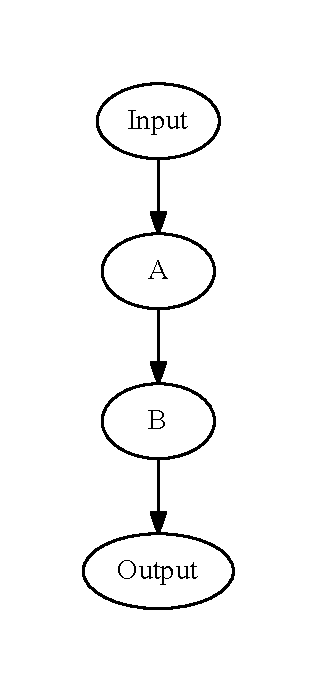
\includegraphics[height=0.2\textheight]{images/TMR-graph.pdf}
        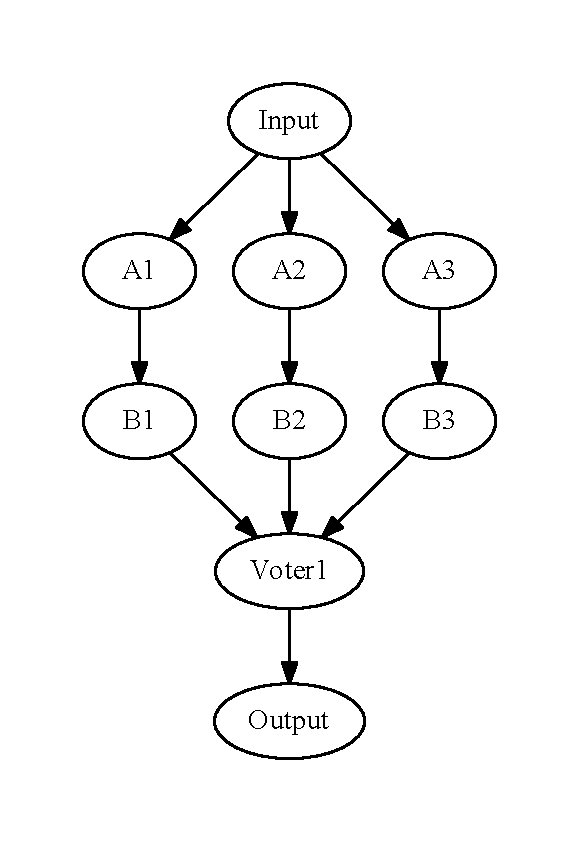
\includegraphics[height=0.2\textheight]{images/TMR-post.pdf}
        \caption{\ac{DFG} before and after partitioning}
        \label{TMRFigure}
    \end{center}
\end{figure}
Given a netlist description of a circuit, it is possible to represent the circuit as a \ac{DFG}\cite{FPGAArch}. Our goal is to split a \ac{DFG} into a number of smaller subgraphs, triplicate the components of each subgraph, and insert voting and recovery logic, with each subgraph having independent components and an error recovery time within our threshold. We can then proceed to implement our graph, made up of our new subgraphs, as normal.
To do so we traverse the \ac{DFG} in a breadth first manner, keeping track of the number of register stages, area, and maximum frequency, extending our partition area as we do so, until our recovery time constraint would be violated. At that point we triplicate our partition, insert our additional voting logic, and then repeat for a new partition, until all nodes have been partitioned.  While doing so we must make sure that no loops exist within a partition and that all values are voted on before being reused, as otherwise the circuit may not resynchronise. This is accomplished by making sure that each node is only added once, and when inserting the voting logic that all outputs are voted on before being used as inputs.

\section{\acs{CAD} Flow}
\acp{FPGA} are typically programmed in a higher level description language such as VHDL or Verilog, and then a number of programs (collectively making up the \ac{CAD} flow or development toolchain) turn the source into a bitstream to program a target \ac{FPGA}.
The design flow process can be split into a number of sub processes as illustrated in Figure \ref{CADFlow}\cite{VPRBook,VPRManual,FPGAArch}.
\begin{enumerate}
    \item The synthesiser turns a hardware description language such as VHDL or Verilog into a netlist of basic gates and flip flops.
    \item The optimiser removes redundant logic, and attempts to simplify logic.
    \item The mapper maps logic elements to primitives, the basic logic elements contained on the \ac{FPGA}.
    \item The packer combines logic elements into \acp{CLB}.
    \item The placer locates each \ac{CLB} within the \ac{FPGA} architecture, deciding which physical block implements which logic block.
    \item The router makes the required connections between each element by deciding which switches are on or off. This includes the connections within each \ac{CLB} (local routing) and in between \acp{CLB} (global routing).
\end{enumerate}

\begin{figure}
    \begin{center}
        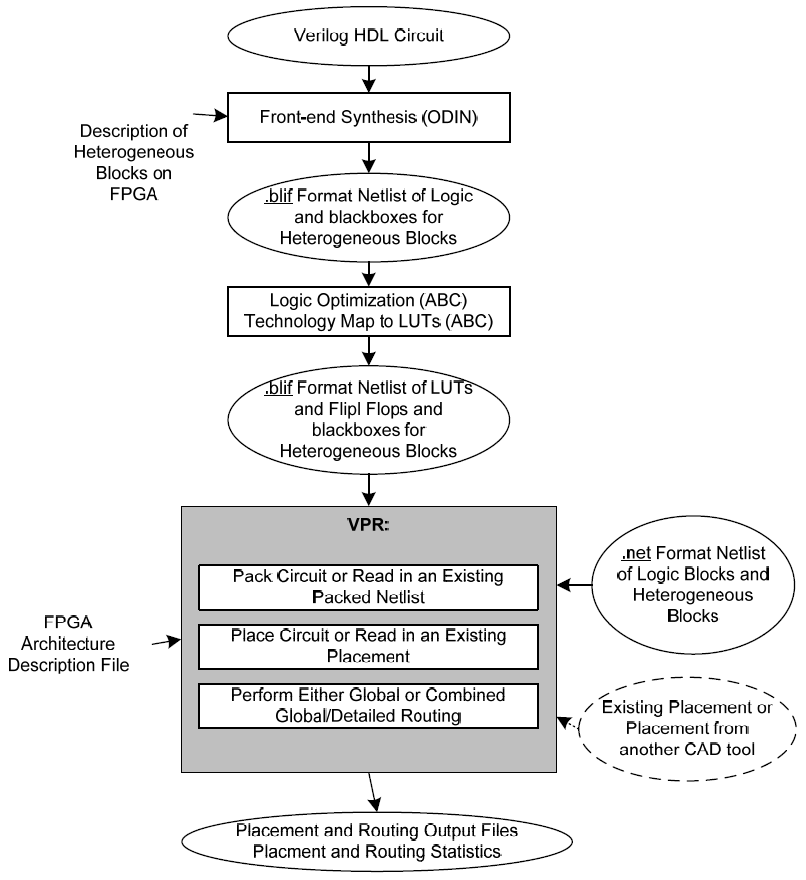
\includegraphics[width=0.75\textwidth]{images/vpr-cad.png}
        \caption{Cad Design Flow.\cite{VPRManual}}
        \label{CADFlow}
    \end{center}
\end{figure}
\subsection{How \acs{VPR} Works}\label{VPRSection}
For this thesis we will be assessing the results of our algorithm implementation after processing by \ac{VPR}, an open source packer, placer and router. \ac{VPR} was chosen as it is open source allowing modifications to be made if necessary, and it is well documented and popular in research, making it much easier for us to determine what's happening and why, rather than relying on proprietary black box processes from commercial vendors.
A brief understanding of the algorithms used in \ac{VPR} and the effects of different settings is useful, though not critical, for understanding the results. \cite{VPRManual} has a more detailed list of all the options \ac{VPR} takes.
\subsubsection{Packer}
\ac{VPR} uses the AAPack algorithm described by \cite{AAPackThesis}. This is a greedy algorithm which operates on blocks sequentially, starting with an \ac{FPGA} area of 1 block by 1 block. For each block it greedily adds primitives based on a configurable cost function until no more primitives can be added. It then repeats for the next cluster, and the next after that, until every primitive is packed. As it runs out of blocks in the current \ac{FPGA} area it expands the \ac{FPGA} area used until it reaches the physical limit specified in the architecture file (or grows indefinitely if no limit is specified). This means that even if the device is of area 40 by 40, if the packer can fit everything in a 30 by 30 area it will do so, and \ac{VPR} will treat the \ac{FPGA} as being only 30 by 30.
The cost function can be configured through options passed to \ac{VPR}, to\cite{VPRManual}:
\begin{itemize}
 \item prioritise optimisation of timing or area (default is prefer timing)
 \item prioritise absorbing nets with fewer connections over those with more (default is yes)
 \item when prioritising absorbing nets with fewer connections, focus more on signal sharing or absorbing smaller nets (default is greatly prefer absorbing smaller nets)
 \item determine the next complex block to pack based on timing or number of inputs (default is timing).
\end{itemize}
The main thing to note, as relates to our results, is that as much as possible AAPack will never leave blocks partially packed. Even when optimising timing exclusively, it will still attempt to maximally pack each cluster.

\subsubsection{Placer}
\ac{VPR}'s placer uses a simulated annealing algorithm where the options allow us to specify annealing schedule parameters and cost function. The default options were chosen via experimentation, are likely superior to custom options we may choose to use, and affect the quality of the result rather than materially affecting the behaviour \cite{VPRManual, VPRBook}. For these reasons we will be leaving them at their default.
\subsubsection{Router}
\ac{VPR}'s router supports three different algorithms:\fxnote{Awkward phrasing, fix} breadth\_first, which focuses solely on routing a design; timing\_driven, the default, which tends to use slightly more tracks (~5\%) than breadth\_first while providing much faster routes (2$\times$--10$\times$) with less CPU time; and directed\_search, which like breadth\_first is routability driven however uses A* to improve runtime. We will be using the default timing\_driven algorithm \fxnote{TODO: Reason?}.
There are a number of options setting algorithm parameters, all of which we will leave at their defaults, though we will be changing the route\_chan\_width parameter as we collect results. route\_chan\_width specifies the width of the channels in the architecture. If omitted \ac{VPR} will perform a binary search on channel capacity to determine the minimum channel width.

\chapter{Benchmarking}
\section{Overview}
\begin{table}
    \begin{center}
        \begin{tabular}{lcccc}
        \toprule
         & \multicolumn{4}{c}{Number of:}\\
         \cmidrule{2-5}
         Name & Inputs & Outputs & Latches & \acp{LUT}\\
         \midrule
            alu4 & 14 & 8 & 0 & 4574\\
            apex2 & 38 & 3 & 0 & 5637\\
            apex4 & 9 & 19 & 0 & 3805\\
            bigkey & 229 & 197 & 672 & 5294\\
            clma & 62 & 82 & 99 & 25177\\
            des & 256 & 245 & 0 & 5018\\
            diffeq & 64 & 39 & 1131 & 4521\\
            dsip & 229 & 197 & 672 & 4283\\
            elliptic & 131 & 114 & 3366 & 10920\\
            ex1010 & 10 & 10 & 0 & 13804\\
            ex5p & 8 & 63 & 0 & 3255\\
            frisc & 20 & 116 & 2658 & 10733\\
            misex3 & 14 & 14 & 0 & 4205\\
            pdc & 16 & 40 & 0 & 13765\\
            s298     & 4 & 6 & 24 & 5796\\
            s38417   & 29 & 106 & 4389 & 18232\\
            s38584.1 & 38 & 304 & 3780 & 18835\\
            seq      & 41 & 35 & 0 & 5285\\
            spla     & 16 & 46 & 0 & 11116\\
            tseng    & 52 & 122 & 1155 & 3260\\
            \bottomrule
        \end{tabular}
        \caption{Benchmark circuits used}
        \label{benchmarkList}
    \end{center}
\end{table}

We have a number of benchmark circuits (detailed in Table \ref{benchmarkList} and obtained as part of the \ac{VTR} project\footnote{\url{http://code.google.com/p/vtr-verilog-to-routing/}}) which we will be using to evaluate the performance of our partitioner and our \ac{TMR} scheme in general.
Additionally, we're looking for ways of estimating area usage and timing information from a \ac{BLIF} file or \ac{DFG}, without needing to actually place and route the partial circuit after each iteration, as doing so is computationally prohibitive.

To start with we made simple test circuits to compare to our benchmarks by triplicating each entire benchmark and adding in simple voter logic. As progress is made on the partitioner we can start collecting results from further partitioned circuits; however triplicating the entire circuit should be sufficient for rough approximations provided $elements_{circuit} >> elements_{voter}$.

To make the test circuits we created a small Python script which, given an input circuit and input voter circuit, triplicates the circuit and adds voting logic. It creates a hierarchical \ac{BLIF} file, that is, it contains nested subcircuits, which are then passed through an external program called \ac{SIS}\footnote{Available from \url{http://www1.cs.columbia.edu/~cs4861/sis/}} to flatten it into a format \ac{VPR} can read.

\subsection{Expected Results}
As is well described in literature (\cite{HardeningTechniques}) and as is intuitive, the area usage should increase by a factor of slightly more than three. There are three copies of each component, plus additional components for the voting circuitry. Maximum frequency is expected to decrease slightly due to the additional components increasing wire length and crowding routing channels however this is likely to vary depending on circuit.

\section{Architecture}\label{ArchFile}
\begin{figure}
    \begin{center}
        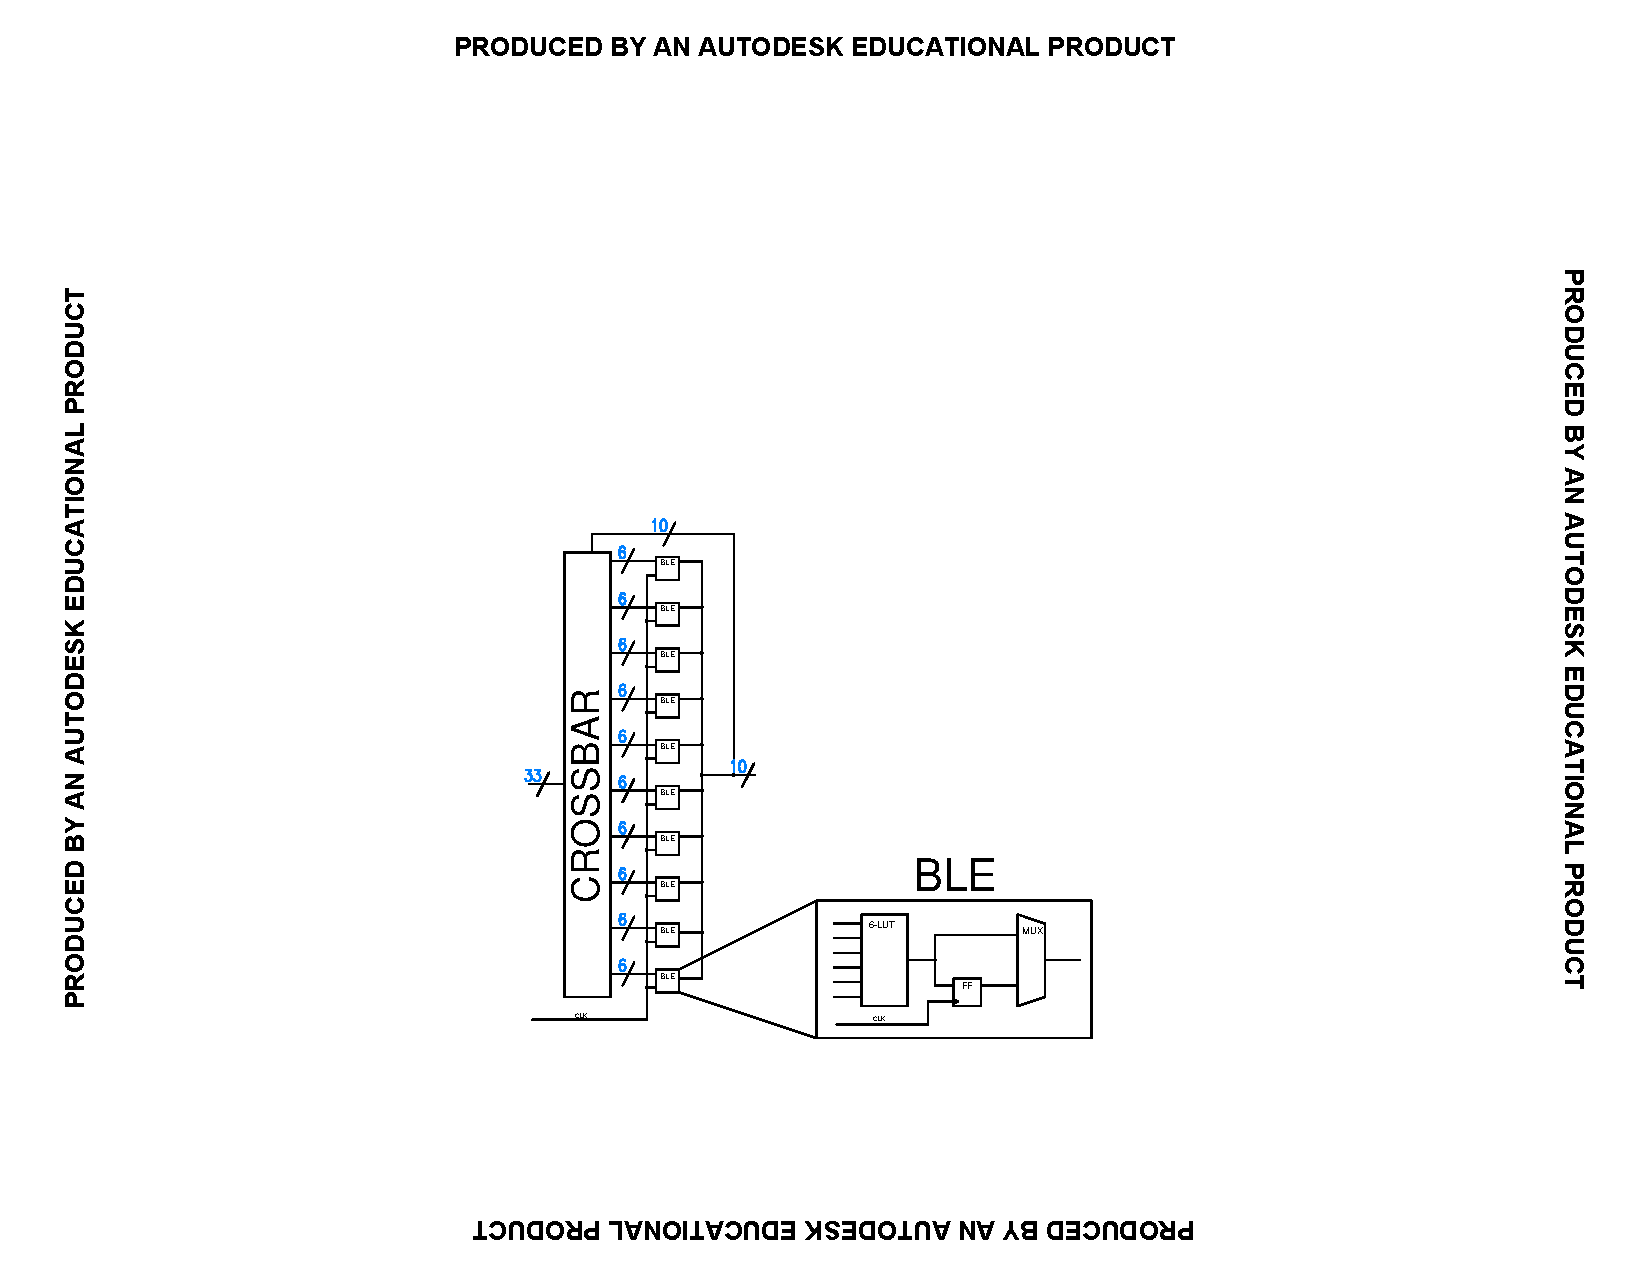
\includegraphics[clip,trim=8cm 4cm 8cm 8cm]{images/CLB.pdf}
        \caption{\ac{CLB} Architecture}
        \label{Arch}
    \end{center}
\end{figure}
\ac{VPR} allows us to specify a custom architecture for it to run against in an XML format. Initially we are keeping the default architecture detailed in \cite{VPRManual} consisting of a grid of \acp{CLB} each consisting of ten fully interconnected \acp{BLE}, and each \ac{BLE} having a latch and 6-\ac{LUT}.
Each \ac{BLE} has 6 inputs and 1 output and each \ac{CLB} has 33 inputs and 10 outputs.


\ctable[
    botcap,
    caption = Architecture Elements,
    label = Arch
]{llll}{
}{
    \FL
    Component & Number & Notes\ML
    Flip Flop & 1 per BLE& Shown as FF on Diagram\NN
    6-LUT & 1 per BLE & \NN
    MUX & 1 per BLE \NN
    BLE & 10 per CLB  &\NN
    Crossbar & 1 per CLB &\NN
    CLB & Autosized by VPR & \LL
}

\section{Methodology}\label{BenchmarkMethod}
To start with, we wanted to collect rough estimates on the impact of partitioning a circuit to provide a baseline with which to compare our partitioning algorithm, and to develop the rough estimates needed for our partitioning algorithm. To that end we first created a simple Python script to take an arbitrary input circuit, triplicate it, and insert arbitrary voter logic. These triplicated circuits were then placed and routed by \ac{VPR}, as were the original benchmarks, and the results compared.

\ac{VPR} is used with our architecture file (described in Section \ref{ArchFile}) and the command line options
\begin{lstlisting}
VPR architecture.xml circuit.blif --full_stats[ --route_chan_width x]
\end{lstlisting} where x is the width of the routing channels and - -full\_stats tells \ac{VPR} to be more verbose in its output.
As mentioned earlier, if - -route\_chan\_width is excluded then \ac{VPR} determines the minimum channel width needed to successfully route the circuit \cite{VPRManual}. We then place and route our benchmark circuits and our partitioned circuits. \ac{VPR} itself then reports the area usage, critical path time (inverse of the frequency), and other statistics we analysed. \ac{VPR} does not unfortunately report the number of register stages however our partitioner will, as it needs to calculate the number of steps for its time estimation function.

\section{Results}\label{BenchmarkResults}
The results listed in this section highlight information of interest in a few key circuits, rather than including page after page of tables. Any aggregate statistics (e.g. median) are calculated on the entire result set, not just the results included. No collected results were considered to be outliers and the only exclusions from the median calculation are those where the operation was not able to be completed, so there is no data.
These tables list scale factors, that is, $\frac{TMR}{Non-TMR}$.
\fxnote{Make this pretty}
\begin{table}
    \begin{adjustwidth}{-1cm}{-1.1cm}
        \begin{tabularx}{1.1\textwidth}{XXXXXXXXXXXXXXXXXXXXXXXXXX}
           \toprule
            Width & Num. Latches & Num. \acp{LUT} & FPGA Width & Channel Width & Num. Wire Segments & Used Area & Frequency & CPU Time\\
          \midrule
            Auto Width         & 300\% & 301\% & 169\% & 119\% & 106\% & 301\% & 93\% & 405\%\\
            200 Width          & 300\% & 301\% & 169\% & N/A   & 110\% & 301\% & 85\% & 385\%\\
            60 Width           & 300\% & 301\% & 169\% & N/A   & 113\% & 302\% & 86\% & 444\%\\
          \bottomrule
        \end{tabularx}
        \caption{Median increase for specified channel widths}
        \label{medianRes}
    \end{adjustwidth}
\end{table}

\begin{table}
    \begin{adjustwidth}{-1cm}{-1.1cm}
        \begin{tabularx}{1.1\textwidth}{XXXXXXXXXXXXXXXXXXXXXXXXXX}
           \toprule
            Name & Num. Latches & Num. \acp{LUT} & FPGA Width & Num. Wire Segments & Used Area & Frequency & CPU Time\\
            \midrule
pdc 200 width   & N/A   & 300\% & 176\% & 104\% & 301\% &  75\% & 425\%\\
tseng 200 width & 300\% & 312\% & 169\% & 126\% & 308\% &  102\% & 388\%\\
          \bottomrule
        \end{tabularx}
        \caption{Increase in circuits with maximum and minimum frequency slowdown}
        \label{timing}
    \end{adjustwidth}
\end{table}
\section{Discussion}
Our simple voter circuit consists of one 3-\ac{LUT} per output. Therefore we expect the number of logic elements (latches and combinational logic) to be exactly three times larger, with an additional 3-\ac{LUT} per original circuit output. As shown in table \ref{medianRes} our triplicated circuits are just slightly over three times as large. Circuit area should be roughly tripled as well, which again, matches, with the width increasing by $1.69 \approx \sqrt{3}$ and the used area increasing by just over triple. The partitioned circuits require slightly larger channels, in order to route the extra wires needed, and the additional elements and wires lead to slightly more segments per wire, and a slightly lower maximum frequency. Of note is that the time to place and route the partitioned circuits was much higher, taking around four times longer.

Circuits were 15\% slower on average, with a worst case of 25\% overall and a best case (in 200 width circuits) of a 2\% speedup. For minimum channel routing the smallest median slowdown was observed as on average the minimum channel width needed for partitioned versions was higher, giving the router more flexibility. For 60 width circuits some were unable to be routed, therefore the results do not represent all circuits. For those reasons the reported statistics are taken from the 200 width circuits.

The speedup, while small, is unusual. It is likely due to the packer having more options, and due to the larger available area (as the packer will only increase the number of \acp{CLB}, and hence \ac{FPGA} area used, when it can no longer fit new primitives in the current block).


\chapter{Partitioning Algorithm}
\section{Overview}
In this section we discuss the partitioning algorithm, including how we are implementing it, progress, and the reasoning behind design choices made.
\section{Design}
We will be implementing the algorithm introduced in Section \ref{Algorithm}, in which we traverse a \ac{DFG} in a breadth first manner splitting the \ac{DFG} into subgraphs which we triplicate and insert voter logic into, while ensuring the error recovery time for each subgraph is below a threshold.

\subsection{Design Choices}
As much as possible, we would like our implementation to be easily extensible to multiple architectures. The actual partitioner operates on a \ac{DFG} so it can be mostly architecture agnostic, only requiring the estimation functions to be architecture aware.
We already have python scripts written to create our benchmark circuits which are able to manipulate \ac{BLIF} files, so we opted for a toolchain incorporating them to reduce development time before we have a working implementation. Specifically, our partitioner operates on \ac{BLIF} files, then generates separate \ac{BLIF} files for each partition, leaving our Python scripts to perform the actual triplication, insertion of additional elements, and stitching them together. Given time we would like to combine the functionality into one program, but this is a lower priority than developing a working implementation.

Other design choices include deciding on \ac{VPR} due to its open nature as discussed earlier in Section \ref{VPRSection}, and how we traverse our \ac{DFG}. A depth first traversal tends to generate long narrow pipelines within each partition, thus increasing the number of register stages, whereas a breadth first traversal lends itself to fewer register stages for the same number of nodes. A possible future improvement is implementing a more advanced traversal algorithm, for example A* with an appropriate heuristic could allow for more elements per partition.

Additionally, we are faced with a choice as to when in the \ac{CAD} process to partition. The closer to the end of the process the more control we have, and the better our ability to estimate area and timing, but the harder it is to partition. As we are inserting new elements we want to partition before packing/placement to allow \ac{VPR} to pack and place our inserted elements.

\subsubsection{Choice of Language}
We are using a combination of languages, mainly Python and C++. Language choice primarily came down to preference regarding familiarity and personal taste although a few other considerations were kept in mind.
For \ac{BLIF} joining and insertion of the voting logic Python was used. \ac{BLIF} files are plain text and the text parsing to join and insert is computationally simple, so the primary concern was short development time while still being readable and maintainable (although Python's performance on text is still quite reasonable)\cite{LanguageBenchmark}.
For the actual partitioner C++ was chosen for a few reasons. Firstly, it was expected that the area and time estimations could be quite computationally expensive, so a lower level compiled language was chosen for performance reasons\cite{LanguageBenchmark}. Secondly, \ac{VPR} is written in C, so using C or C++ allowed for easy code reuse, or merging the partitioner and \ac{VPR}. Our reason for choosing C++ over C was that we preferred an object oriented language as we felt it would be easier to maintain, and would better lend itself to our goal of extensibility, as well as its libraries making our implementation much easier.

\section{Input file format}\label{BLIFSection}
The \ac{BLIF} file format is a textual format which describes an arbitrary sequential or combinational network of logic functions\cite{BLIF}.
Of the full \ac{BLIF} specification, \ac{VPR} only supports a subset of it, and hence our partitioner is also designed to only support that same subset.
\begin{lstlisting}[caption=BLIF file layout, label=SampleBlif]
.model voter
.inputs in1 in2 in3
.outputs out1 out 2
.clock clock
.names in1 in2 in3 out1
11- 1
1-1 1
-11 1
.latch in1 out2 re clock 1
...
commands
...
.end
\end{lstlisting}
\begin{tabular}{lll}
    Model name: & .model $\langle$Name$\rangle$ & The name of the model.\\
    Input List: & .inputs \{Signal\} & The model inputs.\\
    Output List:& .outputs \{Signal\} & The model outputs.\\
    Clock List: & .clock \{Signal\} & The model clocks.\\
    \multicolumn{3}{c}{Commands}\\
    \multicolumn{2}{l}{\ac{LUT}:} & .names \{InputSignals\} $\langle$OutputSignal$\rangle$\\
     &&\{Line\}\\
    \multicolumn{2}{l}{Latch:} & .latch $\langle$InputSignal$\rangle$ $\langle$OutputSignal$\rangle$ [Field ClockSignal] [Field]\\
    \multicolumn{2}{l}{Optional End Marker:} & .end
\end{tabular}

\{Name\} indicates 1 or more of Name. $\langle$Name$\rangle$ indicates a compulsory field. [Name] indicates an optional field.
A combinational logic element (.name) is followed by one or more lines describing the logic function it implements. However, our partitioner only cares about node type and the signals (named with Signal above) as it builds and traverses the \ac{DFG}. All other element information is stored and written back out when the node is written. Likewise for \emph{Field}s.

\ac{VPR} only supports flat \ac{BLIF} files, so only one module declaration is allowed per \ac{BLIF} file. \ac{SIS} can be used to flatten \ac{BLIF} files for use by \ac{VPR}.

\section{Implementation}
Our implementation is still incomplete and so is both liable to change and is not currently match for   our intended design. Most notably, we partition first, then triplicate, then join into one file; not triplicating as we partition. A simple pseudocode description is included in \ref{Pseudocode} (omitting code to read and write \ac{BLIF} files) and is discussed below.

Reading in the \ac{BLIF} file is a relatively simple process as subcircuits aren't supported. We make one pass through the input file, first reading in the list of inputs, outputs and clocks, and then creating a node for each primitive. We then iterate through the set of nodes building a list of signals, with each signal storing its sources and sinks.

\begin{lstlisting}[caption=Simplified Pseudocode,label=Pseudocode]
Model = new BlifModel(file)
Queue = new Queue()
for each(Signal in Model->Inputs)
    Queue.Push(Signal->Sinks)
Partition = new Partition()

while(Queue.Size > 0)
    Node = Queue.Pop()
    if(AlreadyUsed(Node))
        continue
    if(EstimatedRecoveryTime > MAXIMUM_FAULT_RECOVERY_TIME)
        WritePartitionToFile(FileName, Partition)
        Partition = new Partition()
    Partition.Add(Node)
    for each(Signal in Node->Signals)
        Queue.Push(Signal->Sinks)

CombinePartitions()
\end{lstlisting}

As mentioned in Section \ref{BLIFSection}, our input file format is a text file listing all the nodes. We read the file into memory and store it as a \ac{DFG}, with all nodes and signals additionally stored in a hashmap to allow for quick random access. Each node contains a list of all connected signals, and each signal contains a list of all its sources and sinks making the \ac{DFG} quite easy to traverse. Additionally, we store a status for each node indicating whether it is part of the current partition, a previous partition, or new, allowing us to detect feedback loops and avoid adding nodes multiple times.
We then traverse the \ac{DFG} in a breadth first matter while keeping running track of an estimate of the current partition's area and timing information. Once adding a new node would exceed our constraints we write the set of contained nodes to an output \ac{BLIF} file, and proceed with partitioning the rest. Eventually we have one \ac{BLIF} file for each partition. We then pass these to a set of existing Python scripts, written for initial benchmarking purposes and described in section \ref{BenchmarkMethod} which triplicates each partition and inserts voting logic, then connects each partition back up in a hierarchical \ac{BLIF} file. This file is then passed to \ac{SIS} to be flattened, at which point the partitioned circuit is ready for \ac{VPR}.


\section{Estimating restrictions}
As mentioned earlier, in order to partition our circuit we need a method of calculating the partition's (including voter logic) recovery time, which is based on circuit area (affects time to reconfigure), number of register stages (affects time to resynchronise), and frequency (affects time to detect error and resynchronise). Calculating the number of register stages is accomplished while traversing the \ac{DFG}.
Area and timing information are more difficult to determine as they rely on the placement and routing of the circuit. Placing and routing each partial partition every step as we traverse is not computationally feasible in a reasonable amount of time, as placement and routing are relatively slow processes and one of our goals is for our partitioning stage to be approximately as fast as the other stages. Therefore, we need a way of estimating them. To do so we have collected preliminary benchmark information for a number of test circuits and analysed them for patterns allowing us to accurately guess area and timing from a given circuit without placing and routing.

\subsection{Results for Time and Area Estimation}
\begin{figure}
    \begin{center}
        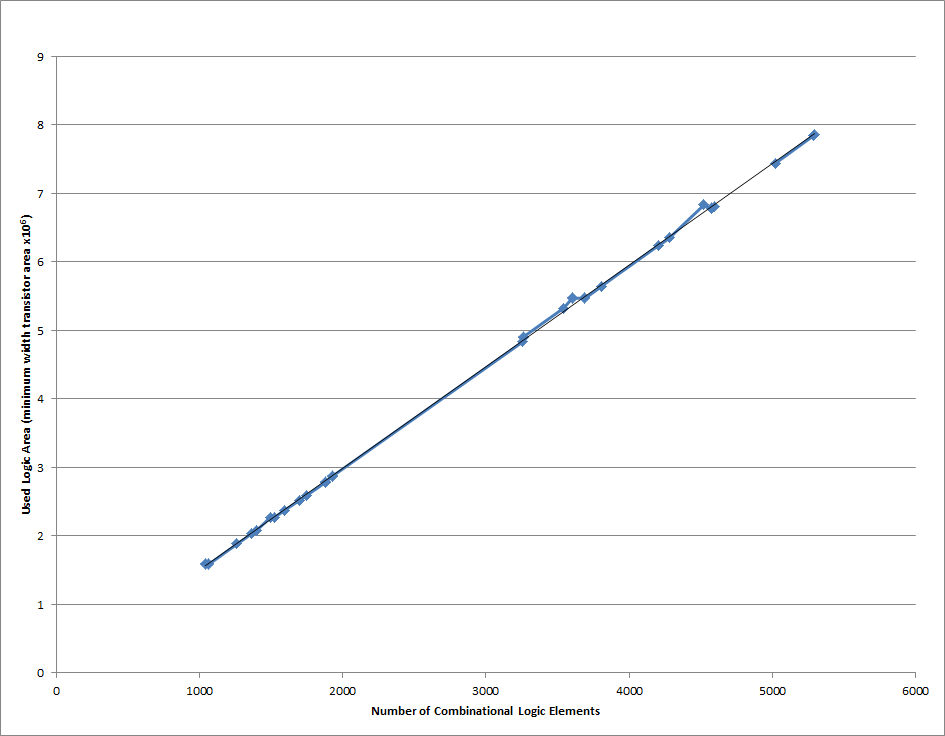
\includegraphics[width=0.7\textwidth]{images/area-v-elements.png}
        \caption{Circuit Area compared to number of Logic Elements}
        \label{AreaVElements}
    \end{center}
\end{figure}


\begin{table}
    \begin{adjustwidth}{-1cm}{-1.1cm}
        \begin{tabularx}{1.1\textwidth}{XXXXXXXXXXXXXXXXXXXXXXXXXX}
           \toprule
            Name & Num. Latches & Num. \acp{LUT} & FPGA Width & Num. Wire Segments & Used Area & Frequency & CPU Time\\
            \midrule
pdc 200 width   & N/A   & 300\% & 176\% & 104\% & 301\% &  75\% & 425\%\\
          \bottomrule
        \end{tabularx}
        \caption{Percent increase in circuit with maximum path slowdown}
        \label{timing}
    \end{adjustwidth}
\end{table}
\subsection{Discussion of Time and Area Estimation}
As shown in Figure \ref{AreaVElements} the area usage can be accurately estimated, as there is a clear relationship between the number of nodes and the area usage. The architecture we are using has one latch and one \ac{LUT} per \ac{BLE}, so for our supported logic elements the number of \acp{BLE} used is close to linear in $max(num_{latch}, num_{names})$. \ac{VPR}'s packer can be either timing or area driven. Currently we are using default settings (mostly area driven) giving us the linear relationship shown in Figure \ref{AreaVElements}; however even when completely timing driven the packer still tries to fill every \ac{CLB}\cite{AAPackThesis}.

After we have a basic partitioning algorithm, an area of further investigation is the impact of changing \ac{VPR}'s settings on the benchmark results, and the accuracy of our estimation functions.

Timing information, on the other hand, is harder to estimate with no obvious pattern, with maximum frequency appearing independent of the number of nodes. In Section \ref{BenchmarkResults} we saw that the median slowdown was 15\% with a 25\% worst result. Conversely, for a few rare cases the partitioned version is actually faster. Initially we will do a rough place and (optionally) route of the original circuit to determine a base time, then multiply it by an experimentally determined slowdown factor to obtain an estimate for the frequency. Initially we are using a slowdown factor of 2 (so half speed after partitioning) which easily encompasses all test circuits we've tried. We can then modify this factor by hand to examine if the impact of it on the final partition's performance warrants improving our estimation function.

\chapter{What next}

\section{Progress}
The initial partitioner implementation is still in progress. We anticipate a basic working version by November 2012, and then will spend the next months collecting results and improving the partitioner.
Done:
\begin{itemize}
    \item Can read a \ac{BLIF} file into a \ac{DFG}.
    \item Can traverse a circuit represented as a \ac{DFG}
    \item Have basic area and timing estimation functions.
    \item Can triplicate an arbitrary circuit (in a single \ac{BLIF} file) and insert arbitrary voter logic (stored in another \ac{BLIF} file).
    \item Initial benchmarks.
\end{itemize}
To Do:
\begin{itemize}
    \item Write \ac{DFG} to \ac{BLIF}.
    \item Incorporate Python scripts into partitioning toolchain.
    \item Benchmark initial partitioning algorithm.
    \item Improve partitioner benchmarks.
    \item Investigate the effect of changing \ac{VPR}'s default parameters upon our results.
    \item Combine functionality of Python scripts and C++ partitioner into one program.
    \item Incorporate that single program into \ac{VTR}'s design flow, likely as part of \ac{VPR}.
\end{itemize}
\section{Schedule}
\begin{figure}
    \begin{center}
        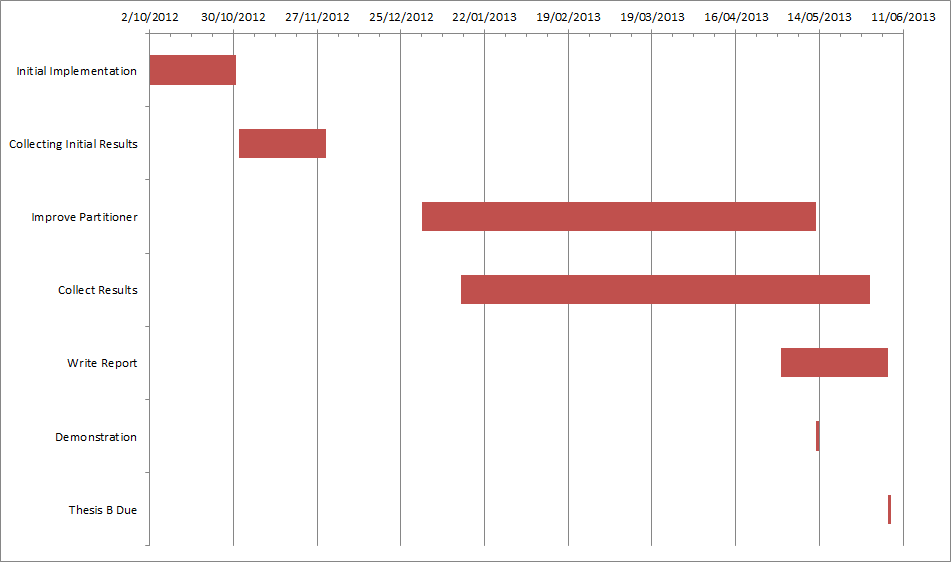
\includegraphics[width=\textwidth]{images/schedule.png}
        \caption{Schedule}
        \label{Schedule}
    \end{center}
\end{figure}

\chapter{Conclusion}
We are currently on track with our initial schedule, and expect to begin collecting results on our partitioner implementation, rather than the effects of generic \ac{TMR}, at the end of this year. During the Christmas holidays progress will likely be quite limited however as we are very close to a working implementation it is believed to be achievable.
Our results collected so far reflect only \ac{TMR} in general, rather than our specific implementation, and they match those of literature and our expectations. We expect slightly worse performance from our partitioner due to additional logic being inserted, but not significantly so.

\appendix
\chapter{Results}
\begin{table}
\footnotesize
\begin{adjustwidth}{-1cm}{-1.2cm}
    \begin{tabularx}{1.1\textwidth}{XXXXlXXXX}
    \toprule
Name & Num. Latches & Num. LUTs & FPGA Width & $\begin{matrix}\text{Channel}\\\text{Width}\end{matrix}$ & Av. No. Wire\newline Segments & Maximum Frequency (MHz) & CPU Time (s)\\\midrule
alu4 & 0 & 1522 & 15 & 200 & 4.76391 &225 & 34.566\\
alu4TMR & 0 & 4574 & 25 & 200 & 5.29148 &188 & 132.41\\\midrule
apex2 & 0 & 1878 & 16 & 200 & 5.5124 &216 & 47.45\\
apex2TMR & 0 & 5637 & 29 & 200 & 6.21459 &172 & 197.825\\\midrule
apex4 & 0 & 1262 & 14 & 200 & 5.0436 &249 & 31.272\\
apex4TMR & 0 & 3805 & 23 & 200 & 5.33318 &204 & 119.002\\\midrule
bigkey & 224 & 1699 & 16 & 200 & 3.70506 &427 & 56.61\\
bigkeyTMR & 672 & 5294 & 27 & 200 & 4.93838 &377 & 193.388\\\midrule
clma & 33 & 8365 & 34 & 200 & 5.62286 &115 & 379.801\\
clmaTMR & 99 & 25177 & 59 & 200 & 6.2762 &103 & 2146.4\\\midrule
des & 0 & 1591 & 16 & 200 & 4.07107 &262 & 98.709\\
desTMR & 0 & 5018 & 27 & 200 & 3.9862 &229 & 263.883\\\midrule
diffeq & 377 & 1494 & 15 & 200 & 3.0611 &157 & 60.103\\
diffeqTMR & 1131 & 4521 & 25 & 200 & 3.44041 &156 & 204.691\\\midrule
dsip & 224 & 1362 & 14 & 200 & 3.823 &433 & 60.372\\
dsipTMR & 672 & 4283 & 24 & 200 & 4.74885 &377 & 177.405\\\midrule
elliptic & 1122 & 3602 & 23 & 200 & 4.2743 &134 & 123.967\\
ellipticTMR & 3366 & 10920 & 39 & 200 & 5.15534 &130 & 513.637\\\midrule
ex1010 & 0 & 4598 & 25 & 200 & 5.31938 &176 & 146.81\\
ex1010TMR & 0 & 13804 & 44 & 200 & 5.4995 &134 & 655.814\\\midrule
ex5p & 0 & 1064 & 13 & 200 & 4.95796 &240 & 30.659\\
ex5pTMR & 0 & 3255 & 22 & 200 & 5.2736 &187 & 112.023\\\midrule
frisc & 886 & 3539 & 23 & 200 & 5.52549 &94.3 & 144.196\\
friscTMR & 2658 & 10733 & 39 & 200 & 5.82234 &90.1 & 525.145\\\midrule
misex3 & 0 & 1397 & 14 & 200 & 4.93 &244 & 35.739\\
misex3TMR & 0 & 4205 & 24 & 200 & 5.46202 &198 & 136.961\\\midrule
pdc & 0 & 4575 & 25 & 200 & 7.21792 &175 & 167.232\\
pdcTMR & 0 & 13765 & 44 & 200 & 7.51339 &131 & 711.155\\\midrule
s298 & 8 & 1930 & 17 & 200 & 4.76794 &124 & 47.789\\
s298TMR & 24 & 5796 & 29 & 200 & 4.83777 &116 & 185.169\\\midrule
s38417 & 1463 & 6042 & 30 & 200 & 3.53974 &158 & 241.471\\
s38417TMR & 4389 & 18232 & 51 & 200 & 3.78557 &149 & 942.7\\\midrule
s38584.1 & 1260 & 6177 & 30 & 200 & 3.67662 &206 & 263.313\\
s38584.1TMR & 3780 & 18835 & 52 & 200 & 4.36338 &157 & 1199.39\\\midrule
seq & 0 & 1750 & 16 & 200 & 5.31333 &253 & 50.624\\
seqTMR & 0 & 5285 & 27 & 200 & 6.23725 &193 & 184.467\\\midrule
spla & 0 & 3690 & 23 & 200 & 6.44786 &190 & 122.311\\
splaTMR & 0 & 11116 & 39 & 200 & 6.75377 &152 & 496.416\\\midrule
tseng & 385 & 1046 & 13 & 200 & 3.04212 &161 & 30.561\\
tsengTMR & 1155 & 3260 & 22 & 200 & 3.82465 &164 & 118.583\\\bottomrule
    \end{tabularx}
    \caption{Results for 200 width channels}
    \label{Results200}
\end{adjustwidth}
\end{table}
\begin{table}
\footnotesize
\begin{adjustwidth}{-1cm}{-1.2cm}
    \begin{tabularx}{1.1\textwidth}{XXXXlXXXX}
    \toprule
Name & Num. Latches & Num. LUTs & FPGA Width & $\begin{matrix}\text{Channel}\\\text{Width}\end{matrix}$ & Av. No. Wire\newline Segments & Maximum Frequency (MHz) & CPU Time (s)\\\midrule
alu4 & 0 & 1522 & 15 & 60 & 4.79098 & 241 & 22.625\\
alu4TMR & 0 & 4574 & 25 & 60 & 5.38017 & 193 & 101.828\\\midrule
apex2 & 0 & 1878 & 16 & 60 & 5.53926 & 212 & 34.256\\
apex2TMR & 0 & 5637 & 29 & 60 & 6.34397 & 164 & 153.485\\\midrule
apex4 & 0 & 1262 & 14 & 60 & 5.13079 & 241 & 20.928\\
apex4TMR & 0 & 3805 & 23 & 60 & 5.66967 & 198 & 90.166\\\midrule
bigkey & 224 & 1699 & 16 & 60 & 3.79333 & 421 & 43.024\\
bigkeyTMR & 672 & 5294 & 27 & 60 & 5.12677 & 363 & 154.662\\\midrule
clma & \multicolumn{7}{c}{Could Not Route}\\
clmaTMR & \multicolumn{7}{c}{Could Not Route}\\\midrule
des & 0 & 1591 & 16 & 60 & 4.15635 & 257 & 50.68\\
desTMR & 0 & 5018 & 27 & 60 & 4.07778 & 230 & 141.366\\\midrule
diffeq & 377 & 1494 & 15 & 60 & 3.20978 & 151 & 28.392\\
diffeqTMR & 1131 & 4521 & 25 & 60 & 3.60614 & 148 & 115.085\\\midrule
dsip & 224 & 1362 & 14 & 60 & 3.84115 & 434 & 36.32\\
dsipTMR & 672 & 4283 & 24 & 60 & 4.87989 & 368 & 118.515\\\midrule
elliptic & 1122 & 3602 & 23 & 60 & 4.76756 & 137 & 101.398\\
ellipticTMR & 3366 & 10920 & 39 & 60 & 5.74891 & 133 & 475.005\\\midrule
ex1010 & \multicolumn{7}{c}{Could Not Route}\\
ex1010TMR & \multicolumn{7}{c}{Could Not Route}\\\midrule
ex5p & 0 & 1064 & 13 & 60 & 5.29429 & 241 & 18.899\\
ex5pTMR & \multicolumn{7}{c}{Could Not Route}\\\midrule
frisc & 886 & 3539 & 23 & 60 & 6.17131 & 94.7 & 107.33\\
friscTMR & \multicolumn{7}{c}{Could Not Route} \\\midrule
misex3 & 0 & 1397 & 14 & 60 & 4.99571 & 241 & 21.286\\
misex3TMR & 0 & 4205 & 24 & 60 & 5.64103 & 197 & 91.433\\\midrule
pdc & \multicolumn{7}{c}{Could Not Route} \\
pdcTMR & \multicolumn{7}{c}{Could Not Route} \\\midrule
s298 & 8 & 1930 & 17 & 60 & 4.62137 & 122 & 27.868\\
s298TMR & 24 & 5796 & 29 & 60 & 4.75444 & 118 & 120.257\\\midrule
s38417 & 1463 & 6042 & 30 & 60 & 3.66998 & 160 & 172.413\\
s38417TMR & 4389 & 18232 & 51 & 60 & 3.87309 & 153 & 758.585\\\midrule
s38584.1 & 1260 & 6177 & 30 & 60 & 3.83166 & 202 & 195.832\\
s38584.1TMR & 3780 & 18835 & 52 & 60 & 4.67375 & 159 & 944.364\\\midrule
seq & 0 & 1750 & 16 & 60 & 5.30778 & 245 & 32.426\\
seqTMR & 0 & 5285 & 27 & 60 & 6.56298 & 188 & 149.187\\\midrule
spla & 0 & 3690 & 23 & 60 & 6.46323 & 188 & 86.03\\
splaTM & \multicolumn{7}{c}{Could Not Route}\\\midrule
tseng & 385 & 1046 & 13 & 60 & 3.22621 & 161 & 20.384\\
tsengTMR & 1155 & 3260 & 22 & 60 & 3.93092 & 164 & 79.889\\\bottomrule
    \end{tabularx}
    \caption{Results for 60 width channels}
    \label{Results60}
\end{adjustwidth}
\end{table}
\begin{table}
\footnotesize
\begin{adjustwidth}{-1cm}{-1.2cm}
    \begin{tabularx}{1.1\textwidth}{XXXXlXXXX}
    \toprule
Name & Num. Latches & Num. LUTs & FPGA Width & $\begin{matrix}\text{Channel}\\\text{Width}\end{matrix}$ & Av. No. Wire\newline Segments & Maximum Frequency (MHz) & CPU Time (s)\\\midrule
alu4 & 0 & 1522 & 15 & 34 & 5.61203 & 196 & 88.236\\
alu4TMR & 0 & 4574 & 25 & 48 & 5.6293 & 182 & 245.343\\\midrule
apex2 & 0 & 1878 & 16 & 48 & 5.78099 & 204 & 80.968\\
apex2 TMR & 0 & 5637 & 29 & 60 & 6.3913 & 167 & 885.343\\\midrule
apex4 & 0 & 1262 & 14 & 48 & 5.74387 & 175 & 55.509\\
apex4 TMR & 0 & 3805 & 23 & 58 & 5.59716 & 181 & 357.909\\\midrule
bigkey & 224 & 1699 & 16 & 42 & 4.00538 & 422 & 84.037\\
bigkey TMR & 672 & 5294 & 27 & 48 & 5.46703 & 351 & 314.02\\\midrule
clma & 33 & 8365 & 34 & 64 & 5.9249 & 111 & 826.48\\
clma TMR & 99 & 25177 & 59 & 74 & 6.81963 & 94.3 & 6225.16\\\midrule
des & 0 & 1591 & 16 & 46 & 4.46904 & 248 & 85.209\\
des TMR & 0 & 5018 & 27 & 44 & 4.43131 & 229 & 329.551\\\midrule
diffeq & 377 & 1494 & 15 & 38 & 3.67617 & 152 & 53.137\\
diffeq TMR & 1131 & 4521 & 25 & 44 & 3.94535 & 156 & 238.817\\\midrule
dsip & 224 & 1362 & 14 & 40 & 4.14675 & 446 & 86.123\\
dsip TMR & 672 & 4283 & 24 & 38 & 5.10172 & 377 & 207.014\\\midrule
elliptic & 1122 & 3602 & 23 & 50 & 5.19297 & 133 & 289.63\\
elliptic TMR & 3366 & 10920 & 39 & 60 & 5.74707 & 133 & 1562.75\\\midrule
ex1010 & 0 & 4598 & 25 & 64 & 5.33384 & 172 & 401.434\\
ex1010 TMR & 0 & 13804 & 44 & 62 & 5.70191 & 131 & 1399.9\\\midrule
ex5p & 0 & 1064 & 13 & 50 & 5.64865 & 229 & 53.45\\
ex5p TMR & 0 & 3255 & 22 & 62 & 6.03046 & 174 & 452.114\\\midrule
frisc & 886 & 3539 & 23 & 56 & 6.66421 & 96.2 & 429.658\\
frisc TMR & 2658 & 10733 & 39 & 66 & 6.5103 & 90.1 & 1383.44\\\midrule
misex3 & 0 & 1397 & 14 & 42 & 5.74857 & 233 & 60.019\\
misex3 TMR & 0 & 4205 & 24 & 50 & 5.86212 & 190 & 368.648\\\midrule
pdc & 0 & 4575 & 25 & 64 & 7.8308 & 156 & 397.958\\
pdc TMR & 0 & 13765 & 44 & 72 & 7.74884 & 121 & 1005.6\\\midrule
s298 & 8 & 1930 & 17 & 30 & 5.16031 & 117 & 2620.11\\
s298 TMR & 24 & 5796 & 29 & 34 & 4.97929 & 119 & 425.303\\\midrule
s38417 & 1463 & 6042 & 30 & 42 & 4.02152 & 158 & 376.671\\
s38417 TMR & 4389 & 18232 & 51 & 50 & 3.96346 & 147 & 7381.12\\\midrule
s38584.1 & 1260 & 6177 & 30 & 44 & 4.22808 & 200 & 459.989\\
s38584.1 TMR & 3780 & 18835 & 52 & 56 & 4.69062 & 156 & 2790.9\\\midrule
seq & 0 & 1750 & 16 & 46 & 5.86111 & 207 & 105.526\\
seq TMR & 0 & 5285 & 27 & 58 & 6.68624 & 190 & 448.058\\\midrule
spla & 0 & 3690 & 23 & 54 & 7.08891 & 144 & 357.396\\
spla TMR & 0 & 11116 & 39 & 66 & 6.92343 & 145 & 1320.57\\\midrule
tseng & 385 & 1046 & 13 & 34 & 3.63807 & 163 & 49.618\\
tseng TMR & 1155 & 3260 & 22 & 42 & 4.36026 & 163 & 183.167\\\bottomrule
    \end{tabularx}
    \caption{Results for autosized width channels}
    \label{Results-1}
\end{adjustwidth}
\end{table}
\bibliographystyle{plain}
\bibliography{../Bibtex/thesis}

\end{document}

%TODO: Tables so they don't split up paragraphs. Table captions at the top? Consistent page numbering? Fix up bibliography. Floats all on one page.
